\section{Find My Disk [Housekeeper]}
\label{test:find-my-disk}

\subsection*{Description}
   The robot helps a blind person to locate a LP, compact disk, or audio-cassette (hereinafter a \textit{disk}) in a shelf. The operator will ask the robot to \emph{describe} what it sees in either the shelf or the media cover, but won't allow the robot to touch her treasures.

\textbf{Main goal:}
   The robot provides a description of an object that matches the operator's requirements.

\textbf{Optional goals:}
\begin{enumerate}[nosep]
	\item Help the blind operator to find a second disk (1000pts)
	\item Provide labeled data (500pts)
\end{enumerate}

\subsection*{Focus}
\HRI{}, \textit{NLU}, \textit{Object Recognition}.


% %% %%%%%%%%%%%%%%%%%%%%%%%%%%%%%%%%%%%%%%%%%%%%%%%%%%%%%%
%
% Setup
%
% %% %%%%%%%%%%%%%%%%%%%%%%%%%%%%%%%%%%%%%%%%%%%%%%%%%%%%%%
\subsection*{Setup}
\begin{itemize}[nosep]
	\item \textbf{Locations:}
		\begin{itemize}
			\item \textbf{Test location:} The test takes place near a bookcase in the living room.
		\end{itemize}
	\item \textbf{People:}
		\begin{itemize}
			\item \textbf{The operator} who is considered to be a blind, and may be blindfolded.
		\end{itemize}
	\item \textbf{Furniture:}
		\begin{itemize}
			\item \textbf{Bookcase:} The bookcase contains at least 10 media boxes placed one next to another, spine out, with no gaps between them. The bookcase door (if any) is open.
		\end{itemize}
	\item \textbf{Objects:}
		\begin{itemize}
			\item \textbf{Disks:} All disks are in their boxes with cover.
		\end{itemize}
\end{itemize}

% %% %%%%%%%%%%%%%%%%%%%%%%%%%%%%%%%%%%%%%%%%%%%%%%%%%%%%%%
% Procedure
% %% %%%%%%%%%%%%%%%%%%%%%%%%%%%%%%%%%%%%%%%%%%%%%%%%%%%%%%
\subsection*{Procedure}
\begin{enumerate}[nosep]
	\item \textbf{Bookcase:} When stored in the bookcase, only the spine of the disk is visible to the robot. The robot can request the operator to pick up a disk and show the cover or back-cover (e.g.~\textit{show me the cover of the first/next disk, please}).
	
		\begin{center}
	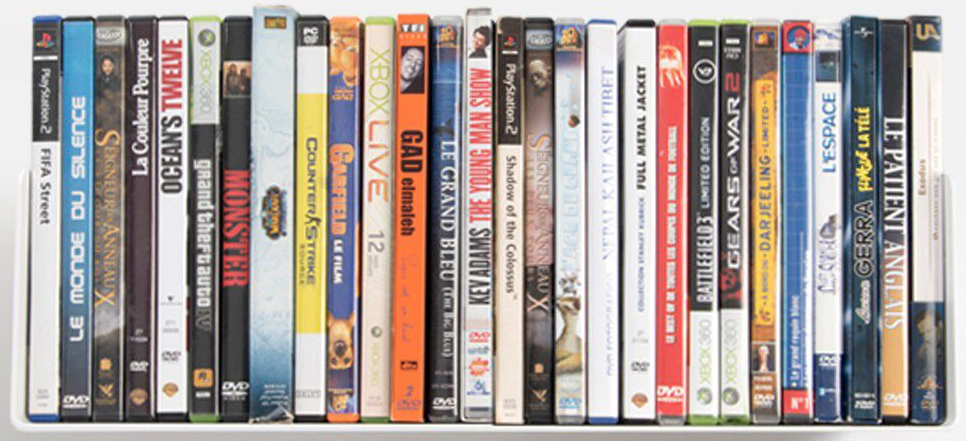
\includegraphics[width=\textwidth,height=3cm,keepaspectratio]{images/find_my_disk.png}
	\end{center}
	
	\item \textbf{Disks:} A \textit{disk} can be the encasing of any CD, DVD, BluRays, audio cassettes, LP, etc. These objects will not be available for training during setup days, although samples can be provided.
	\item \textbf{Test start:} The robot moves to the area near the bookcase where the items are.
\end{enumerate}

% %% %%%%%%%%%%%%%%%%%%%%%%%%%%%%%%%%%%%%%%%%%%%%%%%%%%%%%%
%
% Additional Rules
%
% %% %%%%%%%%%%%%%%%%%%%%%%%%%%%%%%%%%%%%%%%%%%%%%%%%%%%%%%
\subsection*{Additional rules and remarks}
\begin{enumerate}
	\item \textbf{Object manipulation:} All manipulation will be performed by the human operator under the supervision of the robot.

	\item \textbf{Object description and dialogs:} The robot shall provide accurate visual descriptions of the discs in the shelf, and those that are presented to it until the desired object is found. The robot can also lead the interaction by asking relevant questions (e.g.~\textit{what's the cover color?} or \textit{what's the title/author?}), so it can look in the spines and covers as necessary.\\
	It is also acceptable (although not advised), to review each title one by one.

	\item \textbf{Clear area:} The robot may assume that the working area is clear, with no people around making loud noises.

	

	\item \textbf{Data recording:} The provided data must include:
	\begin{enumerate*}[label=(\roman*)]
		\item audio recording of the whole test,
		\item its transcript in plain text format,
		and
		\item a PDF summarizing the interaction.
	\end{enumerate*}
	The PDF report must contain:
	\begin{enumerate*}[label=(\alph*)]
		\item team name,
		\item the audio recording transcript,
		and
		\item each description provided backed with the source image.
	\end{enumerate*}
	
% 	\item \textbf{Deus ex Machina:} The scores are reduced if human assistance is received, in particular:
% 	\begin{itemize}[nosep]
% 		\item human leads the conversation
% 	\end{itemize}

\end{enumerate}

\subsection*{Instructions:}

\subsubsection*{To Referee}

The referee needs to:
\begin{itemize}
	\item Rearrange the disks on the bookcase.
	\item Provide instruction to the operator.
	\item Blindfold the operator.
\end{itemize}

\subsubsection*{To OC}
The OC needs to:
\begin{itemize}[nosep]
	\item \textbf{On setup day}: Provide media samples for practice.
\end{itemize}

% \newpage
\subsection*{Score sheet}

The maximum time for this test is 5 minutes.

\begin{scorelist}
	\scoreheading{Main Goal}
	\scoreitem{1000}{Desired disk is found}

	\scoreheading{Bonus rewards}
	\scoreitem{500}{Provide labeled recorded data}
	\scoreitem{1000}{Help operator to find a second disk}

\end{scorelist}


% Local Variables:
% TeX-master: "Rulebook"
% End:


% Local Variables:
% TeX-master: "Rulebook"
% End:
